\subsection{Events}

\begin{table}[h]
	\centering
	\resizebox{\columnwidth}{!}{
	\begin{tabular}{||c | c | c | c||} 
		\hline
		\textbf{Event} & \textbf{System Response} & \textbf{Source} & \textbf{Type}\\
		\hline\hline
Luminosity detector OFF & Power the lamp & Environment & Asynchronous\\\hline
LED failure detector ON & Notify remote system & Base station & Asynchronous\\\hline
Motion detected & Turn on the lamp & User & Asynchronous\\\hline
Requested to turn on the lamp & Turn on the lamp & Local system & Asynchronous\\\hline
Camera sample & Image processing & Timer & Synchronous\\\hline
Update system information & Send data to remote system & Local system & Asynchronous\\
		\hline
	\end{tabular}
	}		
	
	\caption{Base station events.}
	\label{table:bs_events}
\end{table}


\subsection{Use Cases}
The base station use cases are presented in figure \ref{fig:bs_use_cases}. A street passerby, a car or a pedestrian, can interact with the base station by triggering it's motion detector, or by clearing a parking space.

When movement is detected, the base station lights up the lamp and resquests to the neighbor lampposts to turn their lamps ON. The opposite can also happen, when a neighbor local system, with the lamp already ON, requests the base station to turn ON its lamp. At the same time, in both situations, the information that the lamppost was activated is sent to the remote server. Since the base station is the "primary" station of the network, a third scenario can be put, when there is a local system requesting the base station to turn on the lamp of its neighbor lampposts.

Moreover, the base station is frequently doing image processing through camera frames. So when the street passerby clears a parking space, the system will detect that, sending that information to the remote system.

\begin{figure}[ht] 
	\centering
	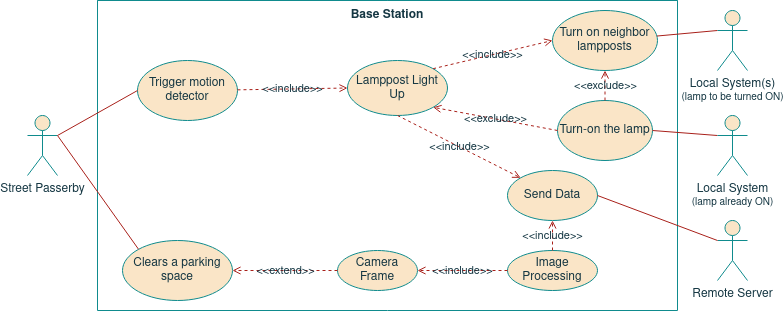
\includegraphics[width=.85\textwidth]{/05base_station/BS_UseCase}
	\caption{Base station use cases.}
	\label{fig:bs_use_cases}
\end{figure}

\subsection{State Chart}
In figure \ref{fig:bs_state_chart} its represented the state chart of the base station. It initiates with system configuration, initializing all subsystems inside the base station, as the Wi-Fi module, sensors data acquisition, image processing. After that, the system enters an idle state. To do the sensors data acquisition, it is used a sample period, that triggers the execution of the function "SampleSensors", detailed in \ref{fig:sample_sensors}. When the base station is requested to turn on its lamp, the lamp is turned-on and a timeout is started. This timeout makes sure that the lamp stays on for more than brief moments. To do the image processing, it is also used a sample period to get image frames through the camera. If there is an available parking space detected, that information is sent to the remote server, as well as when the lamp turns ON.

\begin{figure}[ht]
	\centering
	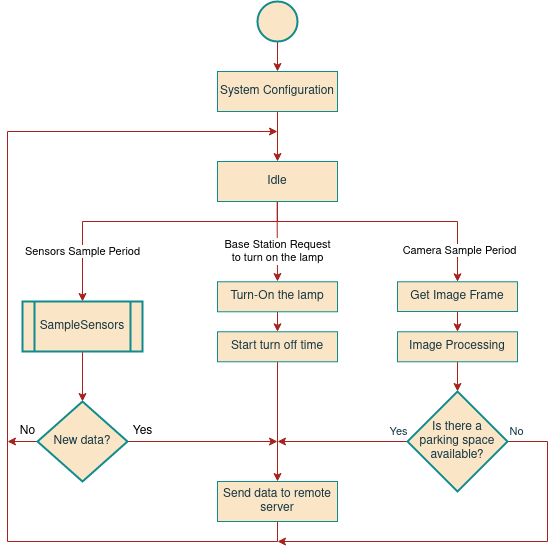
\includegraphics[width=.85\textwidth]{/05base_station/BS_StateChart}
	\caption{Base station state chart.}
	\label{fig:bs_state_chart}
\end{figure}

\clearpage
The sampling of the sensors is represented through the function detailed in figure \ref{fig:sample_sensors}. When low luminosity conditions are detected, through the luminosity sensor, the lamp is powered on, putting the lamp at a predefined minimum bright level. If motion is detected, the lamp is turned on to its maximum bright level, and a timeout is started, as explained before. Besides that, the base station requests the neighbor lampposts to turn their lamps on. When motion is not detected, it is checked if the timeout for the lamp light being ON has already ended. If that is true, the lamp is turned-off. When there is a new information in the system, as when the lamp turns on, that is sended to the remote server.

\begin{figure}[ht]
	\centering
	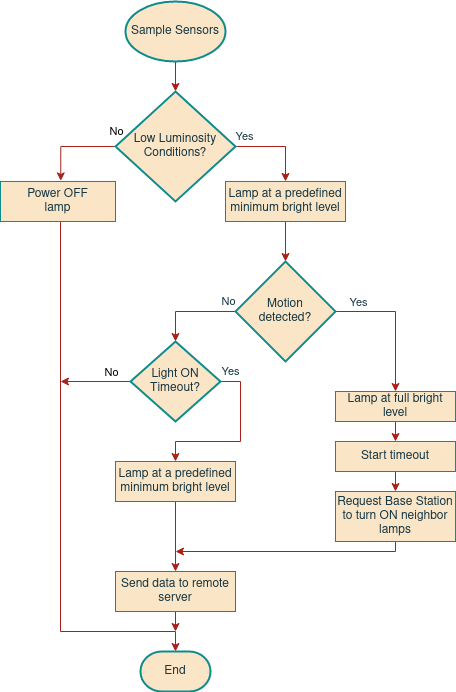
\includegraphics[width=.65\textwidth]{/05base_station/SampleSensors}
	\caption{Sampling of the sensors state chart.}
	\label{fig:sample_sensors}
\end{figure}

\subsection{Sequence Diagram}
In figure \ref{fig:bs_seq_diagram} it is shown the base station sequence diagram. When a street passerby triggers the motion detector, the base station turns on its lamp, and at that moment that information is updated in the remote server. After that, the communication management of the base station is free to communicate with the neighbor local systems to turn on their lamps. If however no more movement is detected, the lamp turns off after a predefined time (turn off time), and again, that information is updated in the remote server.

An alternative of an interaction with the base station is when a local system requests the base station to turn on its lamp, this being processed in a similar way to the previous example.

Finally, the base station can also be requested to turn on the neighbor local systems of the local system that is requesting that.
\begin{figure}[ht]
	\centering
	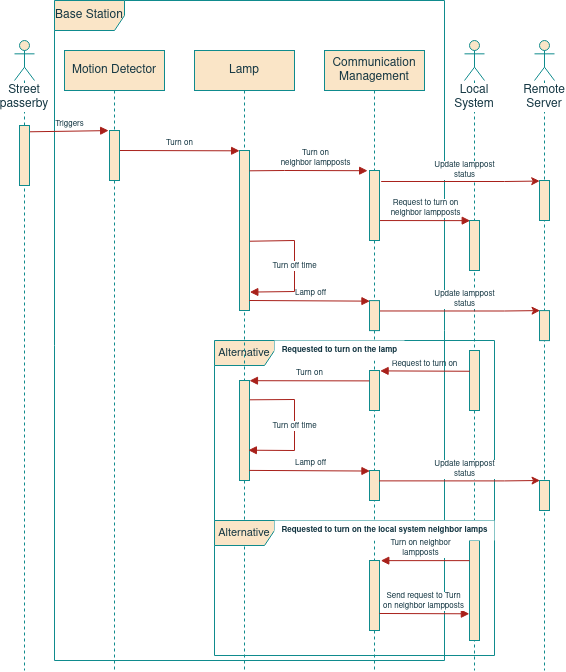
\includegraphics[width=.85\textwidth]{/05base_station/BS_SeqDiagram}
	\caption{Base station sequence diagram.}
	\label{fig:bs_seq_diagram}
\end{figure}